%%%%%%%%%%%%%%%%%%%%%%%%%%%%%%%%%%%%%%%%%
% LaTeX Template
% Version 1.0 
%
% Original authors:
% Hector F. Jimenez S. <hfjimenez@utp.edu.co>
% Brian Ruiz I.		   <brianruiz@utp.edu.co>
% Pereira Security Team 2015.
% License:
% CC BY-NC-SA 3.0 (http://creativecommons.org/licenses/by-nc-sa/3.0/)
%
%----------------------------------------------------------------------------------------
%	PACKAGES AND OTHER DOCUMENT CONFIGURATIONS
%----------------------------------------------------------------------------------------
\documentclass[a4paper]{article} %Formato para hoja A4 Page.
\usepackage[spanish]{babel}      %Seleccion de Idioma Español para las secciones, referencias, etc..
\usepackage[utf8x]{inputenc}     %Utilizamos UTF8 como input.
\usepackage[T1]{fontenc}		 
\usepackage{amsmath}			 %En caso de querer agregar ecuaciones Matematicas.
\usepackage{graphicx}			 %Manejo de Imagenes y formatos.
\usepackage{listings}			 %Se requiere para resaltar codigo de DrRacket
\usepackage{color}				 %Colores.
\usepackage{textcomp}		
\lstset{						%Definicion de Lenguaje a utilizar en los snippets de scheme.
  language=Scheme
}
\usepackage{hyperref}			%Se debe utilizar mejor este
\hypersetup{					%Omite los colores en los hypervinculos.
    colorlinks,
    citecolor=black,
    filecolor=black,
    linkcolor=black,
    urlcolor=black
}
\usepackage[export]{adjustbox}	%Para centering box de imagenes.
\usepackage{geometry}	
 \geometry{
 a4paper,
 total={210mm,297mm},
 	left=30mm,
 	right=20mm,
 	top=20mm,
 	bottom=20mm,
 	bindingoffset=0mm
 }
 
\title{Space Invader V0.7 }
\author{Correo El\'ectronico \\Brian Ruiz, Hector F. Jiménez S.}
\begin{document}
\begin{titlepage} 				%Se encarga de Crear la primer pagina e incluir imagenes.
\begin{center}	  				
\vfill
\line(1,0){320}\\ 				%Lineas Horizontales.Nombre de Desafio y Reto
\huge\textbf{Space Invaders en DrRacket v0.7}\\	
\large{Héctor F. Jiménez S. - Brian Ruiz I.}\\
\large\texttt{hfjimenez@utp.edu.co - brianruiz@utp.edu.co}\\
\line(1,0){320}\\
\large{Pereira Security Team \\Ingeniería de Sistemas y Computación}
\end{center}
\vspace{4em}
\centerline{
\includegraphics[width=\textwidth]{images/logo}} 			
\begin{center}
\large{Universidad Tecnológica de Pereira \\ 2015 }\\
\end{center}
\vspace{7em}																			%Espacio entre imagen e imagen
\centerline{
\includegraphics[width=\textwidth]{images/slice}} 								
\vspace*{\stretch{2.0}}
\end{titlepage}																			%Pagina En blanco
\clearpage
    \thispagestyle{empty}
    \phantom{a}
    \vfill
    \begin{center}Pagina Dejada Intencionalmente en Blanco\end{center}
    \vfill
\newpage
\tableofcontents
\newpage
\clearpage
%\maketitle 				%No se pone pues queda estilo articulo no es la idea.
\begin{abstract}
Fue lanzado en las máquinas recreativas que funcionan con monedas como en la figura (\ref{fig:ejemplo}), el Atari 2600, y la Nintendo Entertainment System. En su vida útil genero más de 500 millones de dólares en ingresos.\\

Es un juego de acción en 2D\footnote{Juego de Accion 2D, https://es.wikipedia.org/wiki/Bidimensional} donde un humano debe proteger la tierra de los extraterrestres. Hay 48 aliens en cada etapa que están uniformemente espaciadas en 6 columnas. Los aliens se mueven hacia izquierda y derecha a través de la pantalla en un patrón establecido, avanzando lentamente hacia la tierra. Es el trabajo del jugador humano disparar a todos los aliens antes de\end{abstract}
\section{Introducci\'on}
Fue lanzado en las máquinas recreativas que funcionan con monedas, el Atari 2600, y la Nintendo Entertainment System. En su vida útil genero más de 500 millones de dólares en ingresos.\\
Es un juego de acción en 2D donde un humano debe proteger la tierra de los extraterrestres. Hay 48 aliens en cada etapa que están uniformemente espaciadas en 6 columnas. Los aliens se mueven hacia izquierda y derecha a través de la pantalla en un patrón establecido, avanzando lentamente hacia la tierra. Es el trabajo del jugador humano disparar a todos los aliens antes de
\section{Proposito del Juego}
El juego Space Invaders ha sido un éxito desde que fue lanzado por Taito en 1978\footnote{Todo acerca de la historia de Space Invaders, http://www.classicgaming.cc/classics/spaceinvaders/history.php}. En el plan original para el juego, era que los aliens fueran a matar a soldas humanos. Taito pensó que no querían enviar el mensaje de que disparar a los  seres humanos  estaba bien, así que lo cambiaron a disparar a los aliens.\\
\begin{figure}
  \centering
    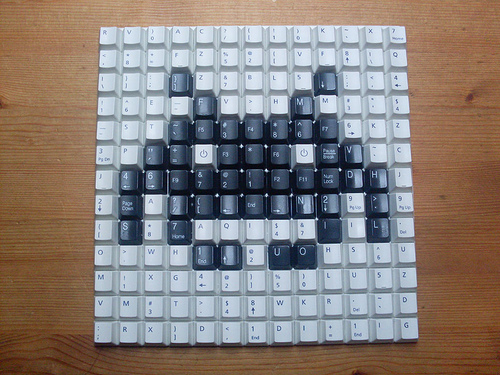
\includegraphics[scale=0.5]{images/spaceinvfun}
  \caption{Arte realizado por un fan.2002}
  \label{fig:arte}
\end{figure}

Poco después de ser liberado, \emph{Space Invaders} creció en popularidad. En 1980, se licencia para su uso en los Estados Unidos. Fue lanzado en las máquinas recreativas que funcionan con monedas como en la figura \ref{fig:ejemplo}, el Atari 2600, y la Nintendo Entertainment System. En su vida útil genero más de 500 millones de dólares en ingresos.\\
\begin{figure}
  \centering
    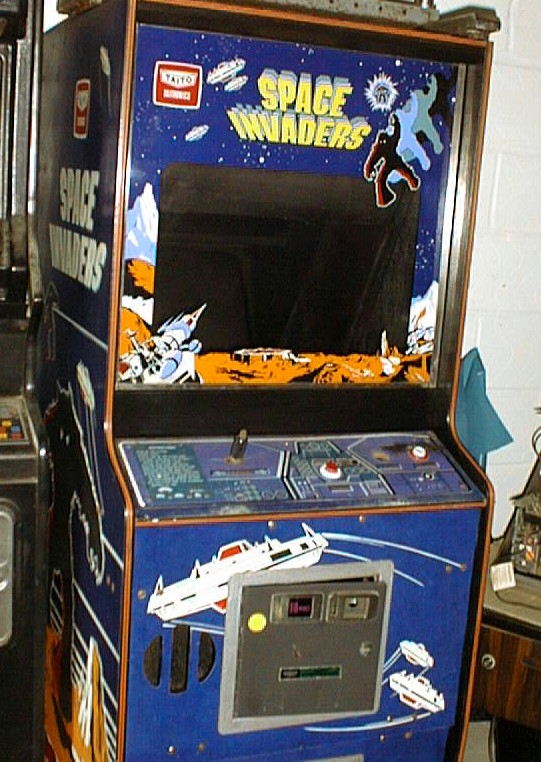
\includegraphics[scale=0.5]{images/machine}
  \caption{Maquina de Space Invaders, Taito 1978.}
  \label{fig:ejemplo}
\end{figure}

\subsection{Principio Basico}
Es un juego de acción en 2D donde un humano debe proteger la tierra de los extraterrestres. Hay 48 aliens en cada etapa que están uniformemente espaciadas en 6 columnas. Los aliens se mueven hacia izquierda y derecha a través de la pantalla en un patrón establecido, avanzando lentamente hacia la tierra. Es el trabajo del jugador humano disparar a todos los aliens antes de que lleguen a la tierra. Los aliens también disparan al azar, por lo que el jugador humano deben evitar esquivar ser fusilado por los aliens. Si el jugador humano es capaz de destruir los 48 aliens, entonces él o ella avanza a la siguiente etapa en la que tienen un nuevo conjunto de 48 aliens para destruir. Otro aspecto del juego es el conjunto de escudos prestados al jugador. En el juego hay 3 escudos que el jugador humano puede utilizar, para  esconderse detrás para evitar recibir un disparo por los extraterrestres. A medida que estos escudos reciben daño, disparos pueden penetrar a través de ellos.\\

Space Invaders se ha actualizado y puesto en libertad en muchas plataformas diferentes, pero todos han sido en forma de dos dimensiones estándar. Hasta el momento Taito nunca ha lanzado una versión en 3D del juego. Sin embargo, en 1999, Space Invaders fue re-lanzado para el Nintendo 64. Aunque los fondos y los personajes fueron diseñados en 3D, el juego sigue siendo un shooter en 2D.

\subsection{Iconos}
En internet existe una gran cantidad de recursos en linea que proveen sonidos, imagenes e iconos, en nuestro caso nosotros solo hemos utilizados dos sonidos obtenidos de aqui\footnote{http://www.classicgaming.cc/classics/spaceinvaders/icons.php} también de \footcite{http://www.softicons.com/game-icons/classic-games-icons-by-thvg/space-invaders-5-icon, SoftIcons} por supuesto se realizan las modificaciones pertinentes para obtener color y transparencias como se puede ver en la figura \ref{fig:iconos}.

\begin{figure}
  \centering
    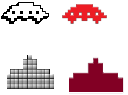
\includegraphics[scale=0.5]{images/iconos}
  \caption{Iconos Utilizados.}
  \label{fig:iconos}
\end{figure}

\section{Requisitos para Correr}

Para correr este juego se debe correr con la opción \textbf{Determine Language from Source}, para que el archivo del juego sea el que seleccione cual sera el lenguaje, para nuestro caso es \textbf{\#lang racket}  ademas de ello solo por seguridad puedes incrementar el limite de memoria de 128MB a 256MB llendo al menu de DrRacket como lo muestra la figura \ref{fig:ml} ,

\begin{figure}
  \centering
    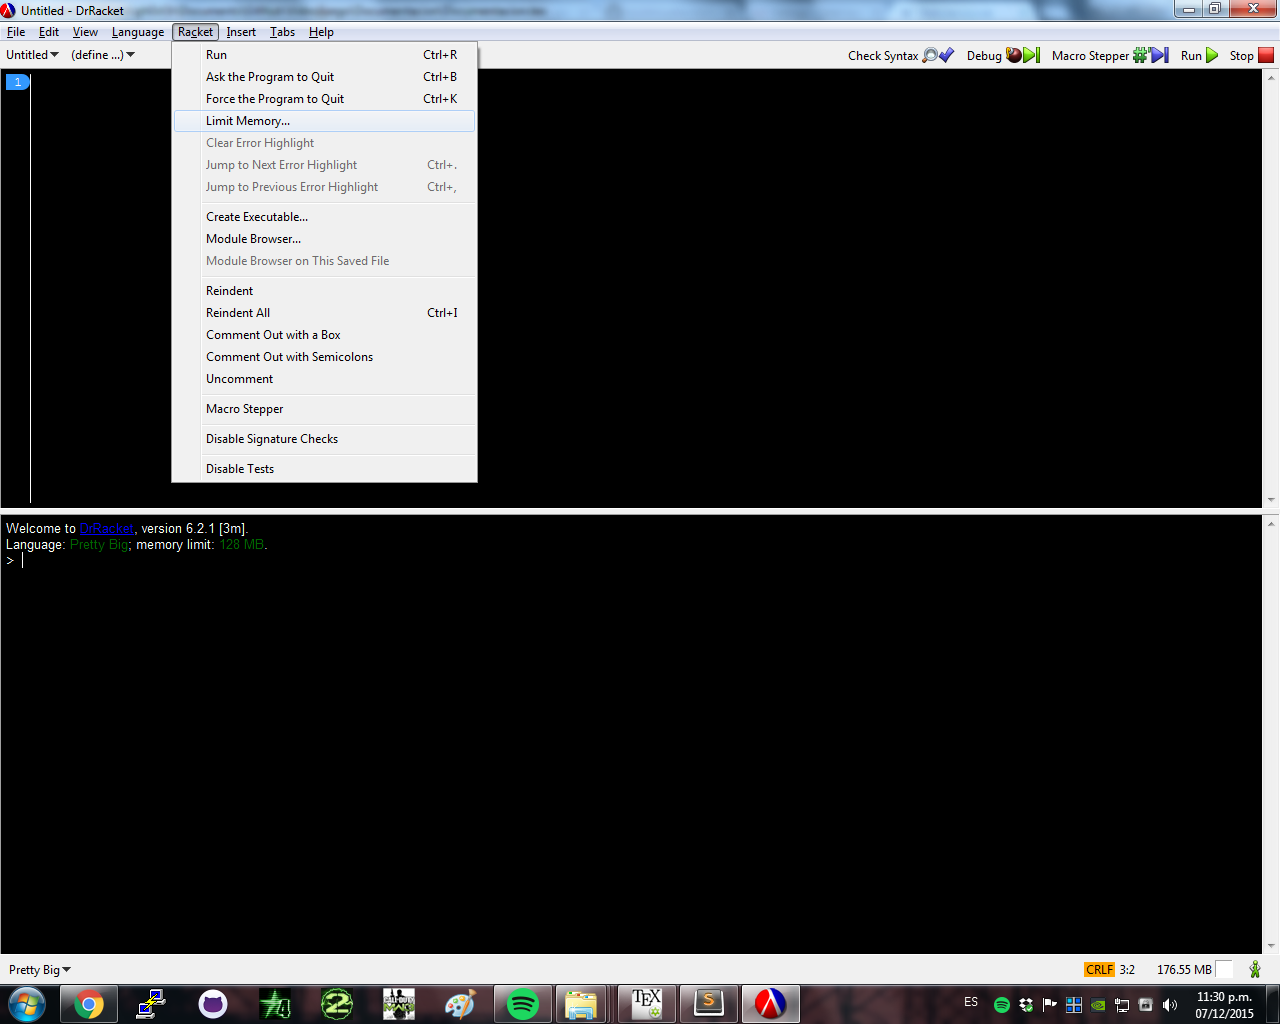
\includegraphics[scale=0.35]{images/limmemoria}
  \caption{Incrementar Cantidad de Memoria en \textbf{\textit{Drracket}}.}
  \label{fig:ml}
\end{figure}

Es estrictamente necesario que las siguientes lineas se ejecuten:
\begin{lstlisting}
\#lang racket
(require 2htdp/image)  
(require 2htdp/universe)
(require math)
\end{lstlisting}

El juego se encuentra \emph{probado} bajo la version 6.2.1 de \textbf{DrRacket} para correr en plataformas Microsoft Windows versiones \textit{ 7,8,8.1,10 Profesional},además  Distribuciones Gnu\/Linux \textbf{\textit{Debian}} y Derivados.
En caso de tener problemas consulte a los desarrolladores.
\begin{figure}
  \centering
    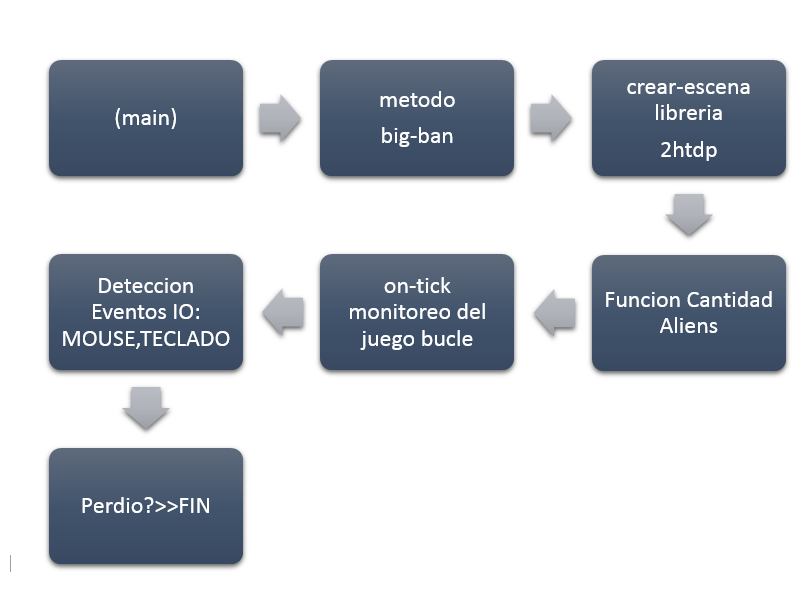
\includegraphics[scale=0.6]{images/smart}
  \caption{Llamado de Funciones, Ciclo infinito.}
  \label{fig:smart}
\end{figure}

\newpage
\section{Detalles Tecnicos de  DrRacket \label{Funciones}}

Para el diseño de este juego y con el fin de poner en practica el concepto de \textit{divide and conquer}, se crearon múltiples funciones, de las cuales se mencionara las mas importantes, además un resumen del ciclo de llamado del juego se puede observar en el siguiente smart art presentado en la figura \ref{fig:smart}, en el cual solamente se ejecuta la primera vez la creacion de escenas, utilizando 2htdp.
siguientes funciones:
\begin{description}
    \item[Comunicador m:] Se encarga de mostrar por pantalla la nave, y enviar los datos a otra funcion denominada \textit{mostrar-balas}
    \item[ver-aliens b:] Se encarga de mostrar los aliens por pantalla, con movimientos.
    \item[monitoreo :]Se encarga de cambiar los valores, también se utiliza para actualizar la posicin de objetos, y crear objetos de manera temporizada. 
    \item[Cambia Posición Aliens:]Actualiza la posición de los aliens dentro de la ventana designada.	
    \item[Mouse] Maneja la posicion de la nave utilizando el mouse, las posiciones de esta solo son en 1d 
        en el eje X, descarta las posicion del mouse en Y,Z.
        
\end{description}

\subsection{Creacion de Ventanas}

\subsection{Funciones de Movimiento}
No olvide Incluir Imagenes.
%http://www.laqee.unal.edu.co/tex-archive/info/epslatex/english/epslatex.pdf
%\begin{figure}
%  \centering
%    \includegraphics{grafico}
%  \caption{Mi Figura}
%  \label{fig:ejemplo}
%\end{figure}

\subsection{Funciones de Disparo}
No olvide Incluir Imagenes.
\subsection{Funciones de Dificulta}
asdasdas
\subsection{Funciones de Sonido}
\clearpage
\newpage
%Toolset.
\section{Links de Paginas de Interés \label{Herramientas}}
\begin{itemize}
\item \href{https://github.com/stuhlmueller/scheme-listings}{Resaltar Codigo Scheme en \LaTeX}
\item \href{www.wireshark.org}{Wireshark}
\item \href{www.wireshark.org}{Terminal Based Wireshark}
\item \href{http://www.gnu.org/software/coreutils/}{Coreutils}
\item \href{http://www.secdev.org/projects/scapy/}{Scapy}
\item \href{http://www.chiark.greenend.org.uk/~sgtatham/putty/}{PuTTY}
\clearpage
\newpage
\section{Agradecimientos}
Agradecimientos en esta seccion \href{http://www.ejemplourl.org}{Ejemplo URL} 

Los autores desean agradecer a esta universidad, al programa de Ingeniería de Sistemas y Computación y al profesor por Francisco por haber asesorado en las consultas y dudas presentadas durante el desarrollo de este juego. Tambien agradecer a todos aquellos que ofrecieron sus opiniones y consejos.
\clearpage
\newpage
\section{Adjuntos}
Archivos Adjuntos: Scripts, Pruebas\ldots etc 


\end{itemize}



\end{document}
%
%|   LOGROS

%tamaño de vantana presonalizable
%fondo e imagenes personalizables con transparencia
%movimiento con raton y tecado
%enemigos en movimiento
%posibilidad de game over

  
%     PENDIENTE
%integrar sonidos
%poder matar a los enemigos
%poder adicionar enemmigos



% MANUAL DE PROGRAMADOR, Esto ira en el manual se eliminara cuando el manual este completo.
%Manual esta hecho en latex.
%Este codigo necesita mas de 128Mb de ram, preferiblemente incremente la memoria.a 256Mb.
%ok
%lenguaje --> lang racket

%El mundo se utiliza para que barias funciones interactuen simultaneamente 
%y se puedan embiar parametros de una forma facil, la funcion principal 
%(big-bang) embiala actualizaciones contantemente a cientas funciones,
%la estructula para usar es: 

%(define-struct identificador [rama1 rama2 ....])

%(big-bang identificador
%[aqui-caracteristica-a-emplear mi-funcion]
%[aqui-caracteristica-a-emplear mi-funcion2]

%big-bang embia todos los datos a las funciones secuencialmente

%para extraer los valores del mundo que definimos ariva hacemos 
%el llamado de cualquiera de las siguentes funciones
 
% (mundo-jugador a)
% (mundo-disparo a)
% (mundo-enemigos a)   )

%para cambiar balores del mundo se usa (make-mundo  _ _ _ ) y en las lineas se mencionan los nuevos 
%Bibliografia

%iconos--> 
